\documentclass[]{article}
\usepackage[pdftex]{graphicx}
\usepackage[top=1in, bottom=1in, right=1.25in, left=1.25in]{geometry}
\usepackage{hyperref}
\hypersetup{colorlinks=true, linkcolor=blue, urlcolor=blue}

\begin{document}
	\tableofcontents
	\newpage
	%39th Entry
	\section{Compilation Work with Phil (04/11/2013)}
	
	Worked with phil for a few hours to get the latest image cleaning software integrated with the rest of the analysis program. Finally got it to work. Note to self: always ensure that you have something else to do when each debug run takes 6 minutes.
	
	%38th Entry
	\section{Website updating (04/??/2013)}
	
	Updated the website's demonstration page to reflect the latest progress on our project.
	
	%37th Entry
	\section{image cleaning with color  (03/30/2013 and 04/04/2013)}
	
	My job for the past week has been to get the image cleaning software working with colored markers. Towards this end I had a couple options: I could use the YCbCr color coding, which comes with its own grayscale values or I could use the RGB encoding and calculate the grayscale based on the RGB values. After looking into YCbCr a bit I decided to stick with RGB because I am more familiar with it and because my code was already opening them in RGB. 
	
	After looking at various ways to clean the image based on RGB values I eventually decided to stick with what I already know how to do. I went through each stroke cell and analyzed it pixel by pixel. If the pixel's grayscale value (calculated from its RGB values) was less than the avg grayscale value I made it pure white, else I left it alone.
	
	The results (once I got the code to actually work.....) are surprisingly good: \\
	
	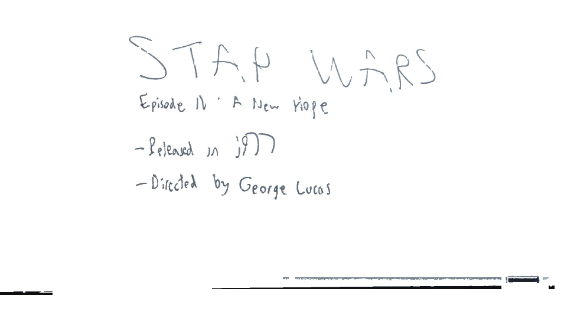
\includegraphics[scale=1]{images/Color1.png} \\
	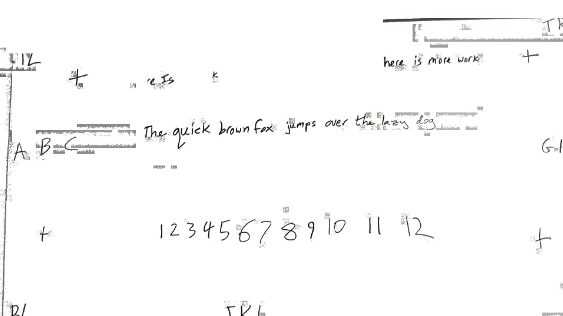
\includegraphics[scale=1]{images/Color2.png} \\
	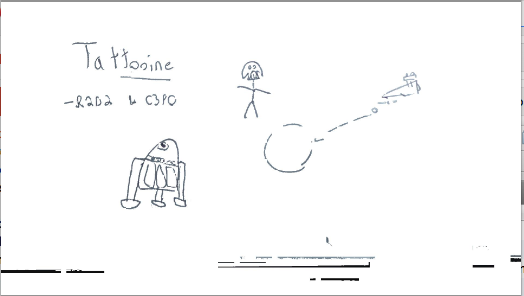
\includegraphics[scale=1]{images/Color3.png} \\
	
	I realize that the past three images had black markers, but decided to show them because they are in our current testbed of images. Here is an image with colored markers. Please ignore all the mis-classified cells! :D \\
	
	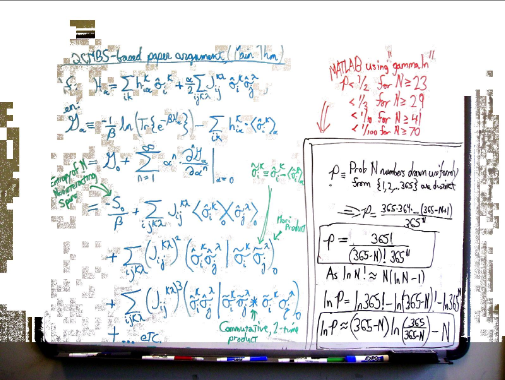
\includegraphics[scale=1]{images/Color4.png} \\
	
	%36th Entry
	\section{more work image cleaning 03/28/2013}
	
	Today's work focused on further cleaning up the images and on identifying further problems. I cleaned up the images a little more by modifying the dynamically calculated threshold value. I originally calculated this value by finding the average grayscale value within the cell. This value was actually a little too hight, so to compensate i decided to subtract the standard deviation of all the cell values from the average. I decided to do it this way only after several hrs of research/browsing. I needed something that would vary from cell to cell based on the distribution of grayscale values, but i also needed it to be small enough that I wouldn't completely throw off my averaging. As it so happened, this standard deviation value, while varying from cell to cell, was a little too high, so I divided the stddev by 5. This seems (from the photos I've tested so far) to be the right number. It may need to be adjusted for more extreme images.
	
	Before further cleaning: \\
	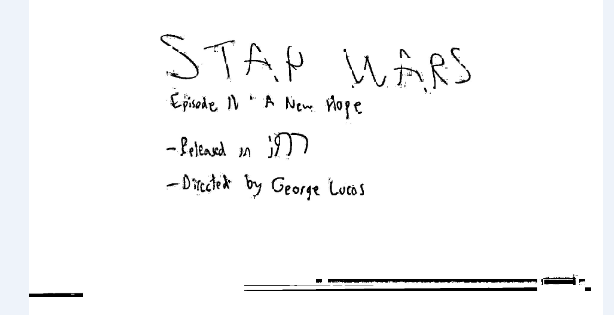
\includegraphics[scale=1]{images/withoutStdDev.png} \\
	
	After cleaning: \\
	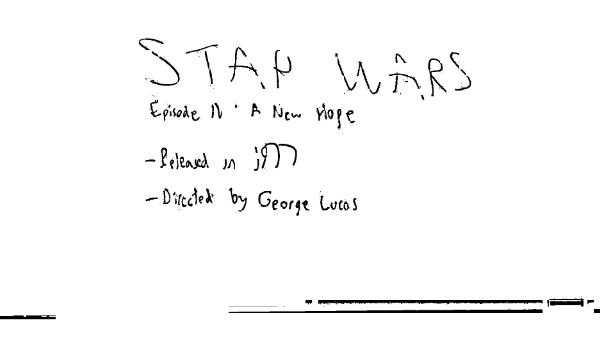
\includegraphics[scale=1]{images/withStdDev.png} \\
	
	Remember that this is still run with the old cell classificationsoftware. Better classifications would capture all pieces of the letters.
	
	While testing I noticed a few cases where cells had been misclassified as stroke cells. This is currently not good for my program because it adds unnecessary black to the image:
	
	Misclassified Cell Image: \\
	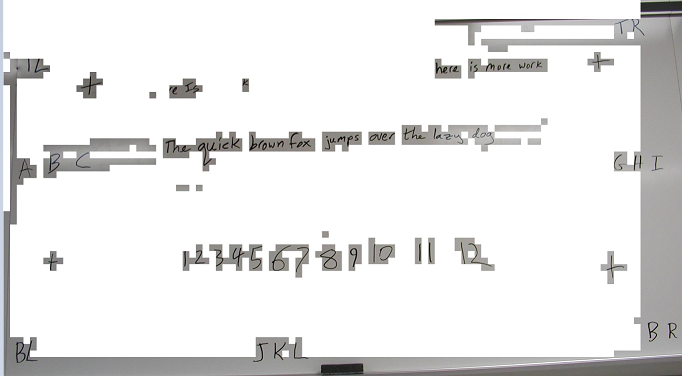
\includegraphics[scale=1]{images/Misclassify.png} \\
	
	Misclassified result: \\
	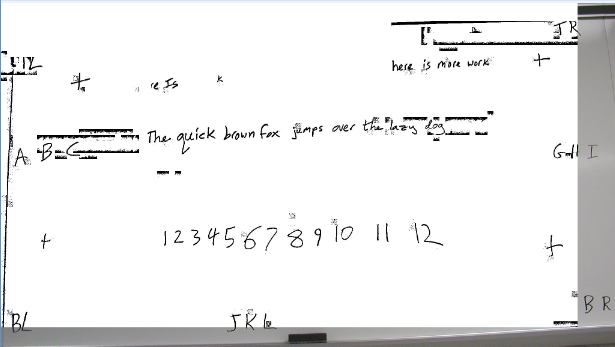
\includegraphics[scale=1]{images/misClasResult.png} \\
	
	Notice how the misclassified results tend to leave dark patches on the image.  Below is another example. It both shows how well the program works when the strokes are correctly classified and how poorly it deals with misclassified cells: \\ 
	
	Before: \\
	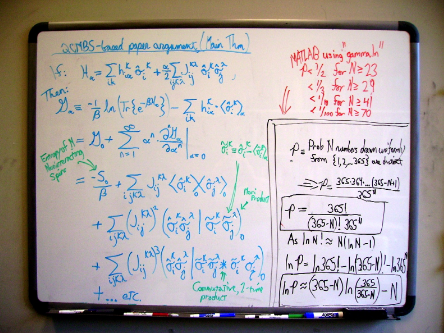
\includegraphics[scale=0.75]{images/origMisBord} \\
	
	After: \\
	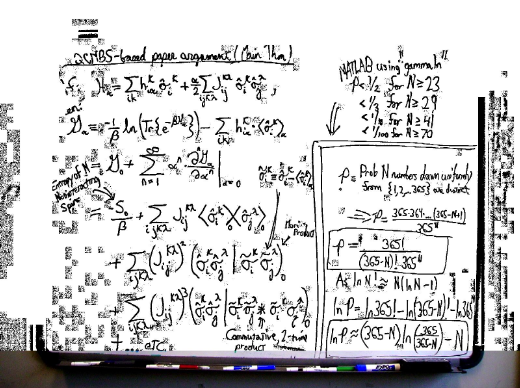
\includegraphics[scale=0.90]{images/bordWMisses} \\
	
	
	%35th Entry
	\section{Image cleaning work 03/26/2013}
	
	Today's work focused primarily on the cells that had been classified as stroke cells. My goal was to make each stroke cell into a 2 bit image. This way (I hoped) I would be able to work around/remove the changing brightness issues discussed in previous entries.
	I think just showing the images explains it all:
	
	Original: \\
	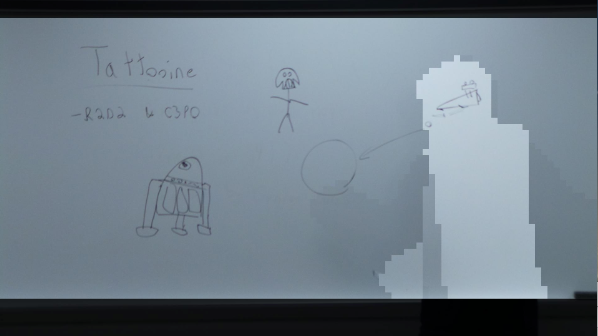
\includegraphics[scale=1]{images/Orig.png}
	
	White Background cells: \\
	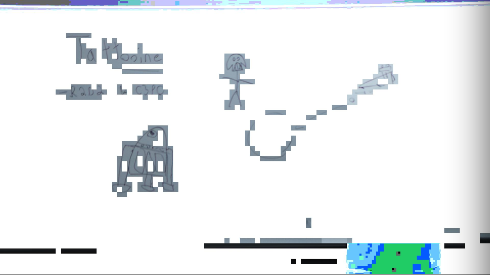
\includegraphics[scale=1]{images/WhitBack.png}
	
	Static: \\
	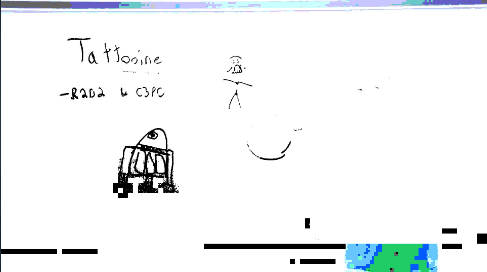
\includegraphics[scale=1]{images/Static.png} \\
	
	
	As you can see, even with smaller areas, using static threshold values isn't going to work.
	I then looked into various ways of finding the average grey value of a given image. When I found one that worked I implemented it:
	
	Best so far: \\
	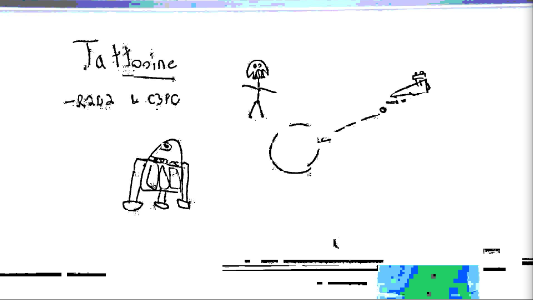
\includegraphics[scale=1]{images/Best.png} \\
	
	If you notice, there are gaps in the lines of some portions of the drawing. This is because I was using old cell detection software which missed some of the stroke (look closely at the "White Background cells" image to see what I mean).
	
	I am pleased with my progress so far...though I'd like to get the accuracy down a bit more before our final product because there are still quite a few errors. I think something that might improve further accuracy will be to find the most common greyscale color value rather than the average greyscale. The average starts mis-classifying when the difference between the board and the stroke is very slight. We shall have to see how much better the common greyscale value is though.
		
	%34th Entry
	\section{Image cleaning work 03/20/2013}
	
	I worked to create 2-bit images today.
	In this process I first converted each image to grayscale (16-bit grayscale). I then defined a threshold and if a pixel was darker than the threshold it was set to pure black and if it was lighter, it went to pure white. This method would have worked perfectly if the board had a uniform background color. Unfortunately, the non-uniform lighting means that some areas of the board are darker than others. Thus a dark board cell on one side of the image often became pure black whereas a black stroke/line on the light side of the board became pure white. What I'll have to do is make decisions based on the color of surrounding cells/pixels rather than the board as a whole so that the conversion process takes into account relative darknesses.
	%33rd Entry
	\section{Image cleaning work 03/15/2013}
	
	Today I focused primarily on stroke cells. I ran Colin's code to determine which cells had writing in them, and turned all other cells white. As you can see below, while this did a great job isolating the cells, it hasn't gotten me any closer to fixing up the white/gray cells that surround the handwriting.
	
	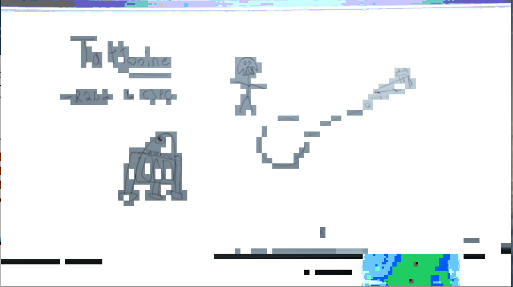
\includegraphics[scale=0.5]{images/Cells1.png}
	
	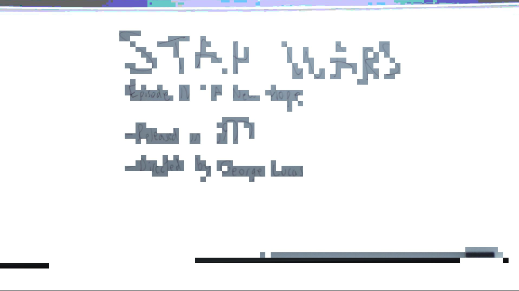
\includegraphics[scale=0.5]{images/Cells2.png}
	
	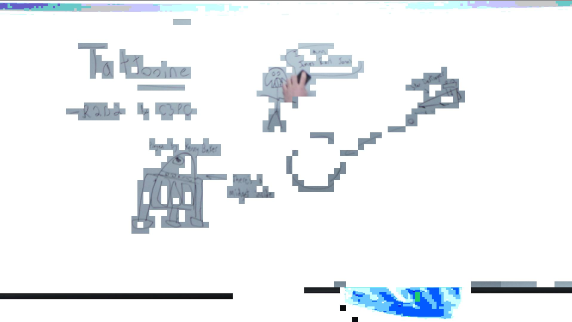
\includegraphics[scale=0.5]{images/Cells3.png}
	
	I tried to increase accuracy by increasing the number of cells in each image but this exponentially increased the processing time and did not noticeably improve the quality of the final images.
	
	%32nd Entry
	\section{Image processing work 03/10/2013}
	
	Today I re-familiarized myself with my previous work on image cleaning. I worked for a while with the openCV framework that I'd researched extensively in the beginning of last semester but finally decided that the filters offered weren't useful enough to justify using. I then went back to the regular PIL and made some progress. The main roadblock I hit is the fact that the filters rely on a uniform background brightness whereas our stitched together images come in many shades of gray. I decided that I should probably take a new approach when i get back to this. When I work next I think I will try creating two-bit images (pure black or pure white) and I will also look into setting non-stroke cells white automatically so I can just concentrate on the stroke cells.
	
	
	%31st Entry
	\section{Website Improvement 02/28/2013}
	
	I updated the website today. We decided to create a demonstrations page for our website.
	There is now a youtube video of colin setting up the camera in well under 5 minutes, as well as a series of images demonstrating our progress on the image processing software. We decided to add more to our website after looking at our panel 4 feedback. 
	
	I also did more research on image filtering. After looking through my past research I brainstormed more ways to make the final images look good. The goal is to have a pure white background with pure black/color text. It seems like the easiest initial step will be to go cell by cell on the key images. If it is a stroke cell, leave it alone, else color it pure white. This will get rid of most grayness. There will still be grey around the text however. 
	At that point we'll be left with a decision: do we want manual adjustment or auto-adjustment. Automatic would be the ideal situation obviously, but auto-correction might not be as effective/good looking.
	I'd say that for now we should assume auto. With that in mind, for the stroke cells, it will likely be easiest to simply look at each pixel. If it is a gray value (within a threshold) then make it white, else make it pure black. This would work for most professors, but some like using colored pens. in this case it would be the same, but if it isn't the gray values then leave it alone.
	
	I looked into keystone imaging again. I didn't find anything that matched our needs perfectly, but I"m confident I'll find something if I keep looking. I didn't look very long because I had other work to do but there were quite a few sites that described exactly how it works...the tricky part will be finding the right python example.
	
	%30th Entry
	\section{Client meeting 02/25/2013}
	
	Phil and I met with Dr. Midkiff today to discuss our fourth panel. He was pleased with our progress and happy to see how far we'd come since our last client meeting. See the minutes for this meeting for more details.
	
	%29th Entry
	\section{Groupwork on image capturing and lighting 02/22/2013}
	
	We spent several hours attempting to (programmatically) set manual parameters for our camera before image capturing. We wanted to stop it from auto=adjusting its settings during image capture because it changes the overall lighting of the pictures. This is bad because our image capture system relies on a steady background brightness. When the professor steps into the middle of the shot, and then moved away, the camera was compensating, and the images got very yellowed from that point onward. We could not figure out how to manually access the ISO, shutter speed, and aperture, so instead we've taken to messing with other settings. We attempted to have the cameral only make adjustments if the top rim of the photo's light/brightness changed. Unfortunately the program seems to be ignoring some of the commands we give it. Strangely some commands do work, so it's been rather hit or miss so far.
	
	Update: It looks like phil has changed the math behind the stroke detection algorithm so we no longer need the steady brightness like we needed before. It looks like at this point I should start looking back into the image processing software I'd been researching earlier because as soon as the detection is complete it will be time to make the image "pretty" (make the white board a true white, keystone imaging (to adjust for angled images) etc.
	
	
	%28th Entry
	\section{Client meeting 02/22/2013}
	
	We met with Dr. Gabauer today to discuss our progress so far and to summarize the parts demonstration that he was unable to attend. He was pleased with our progress and excited to see how our final product. He asked what we thought about capturing two whiteboards with the camera (zoom out more) and we said we'd look into it. It all depends on how much detail we can capture from the board while zoomed out that far. Another suggestion was that we might consider setting the board's boundaries using the Galaxy Camera's large touchscreen during setup. We're going to look into this as well because this selection would give us a couple options: it might allow us to only photograph certain portions of the board. If that doesn't work, it could at least give us four coordinates on the pictures, so that we can auto-crop them on the back-end, before the actual image processing begins.
	
	We will be meeting Dr. Midkiff on monday (02/25/2013) to discuss our panel results and receive feedback from him as well.
	
	%27th Entry
	\section{Parts Demonstration}
	
	I was rather disappointed by the parts demonstration today. I was under the impression that we would be demonstrating the functionality of our project to date, and that we would then receive comments on our progress, and maybe a tip or two if we were having trouble implementing our plan.
	
	Instead, we were grilled the whole time about portions of our project that we weren't even closed to finished with yet. It became a critique session rather than a dialogue about our process so far. I also noticed that the professors with the most criticism and questions were the professors who weren't familiar with our documentation. The parts demonstration should not have been focused on how we have implemented our product so far. That implementation is described very clearly in our reports from last semester, our work logs, etc.	
	
	There were a few questions about the capture system, a couple about out automation system, but the majority were focused entirely on the image processing. One could argue that the image processing is the most important part, but in order to get there we had to get everything else working. We are now focusing more on the processing portion and we've made big leaps since last semester. 	
	%26th Entry
	\section{Individual work on deamon}
	
	I spent a little time working on making the comments/functionality of the Deamon work better for our parts demo. 
	
	% 25th Entry
	\section{Individual work on process automation 02/07/2013}
	
	I spent many hours today working on my python deamon/process automation combo. I felt bad because I hadn't done very much work over the past week, so I put in extra work today.
	
	Today's achievements: I created a deamon that checks a given folder every 5 seconds to see if there are any files in it. If there are, it moves them to another folder for further processing. We are now ready to take the processing code that phil/colin have been working on, and auto-run it on whatever files are placed in the picture-submission folder.
	
	Aspects of my work that took significant amounts of time:
	
	\begin{itemize}
					\item Getting deamon running initially.
						\subitem{This took time because i was still getting ahang of the basic deamon layout. once I had it figured out, the actual implementation didn't take too long.}
					\item Finding the new files and saving their names using diff and ls
						\subitem{This took time because once I had to figure out how to both get the names, remove the extra text that diff adds on, etc}
					\item Combining items 1 and 2.
						\subitem{This took a long time because i forgot how finniky Python can get if you mess up with tabs/spaces. I eventually ended up re-typing the whole program because I couldn't find where my spacing was causing my deamon to crash.}
					\item Moving files between directories using the names supplied by ls and diff
						\subitem{This took an embarrassingly long period of time to actually implement. I couldn't figure out why my various implementations kept failing. I finally discovered that it was because i wasn't removing the line end character from my string before adding it to the source address.}
	\end{itemize}
		
	I am happy to report that we're now ready to demonstrate our working deamon as it moves files from a source folder to a destination folder.
	Looking back i see that it would have been easier to simply make a method that returns true if there are files in the given folder. I could then have simply moved everything with one command. I like my implementation (moving files on a name by name basis) because it will be more useful later when we might not want to move all files in a specific folder.	
	
	
	% 24th Entry
	\section{Individual work on deamons 02/04/2013}
	
	Today I spent time implementing various pieces of my deamon/process automation research from 1/27.
	I made a script with python that created a file containing all new files in a folder using a combination of ls and diff.
	Since we'd decided to create our own python deamon in last week's meeting I did some further research on creating deamons in python. I found another site that had a good python deamon example in it, and I plan to try using it to create my own custom deamon.
	
	\url{<http://code.activestate.com/recipes/278731-creating-a-daemon-the-python-way/>}
	
	% 23nd Entry
	\section{Group Work with Phil on our Linux machine 01/31/2013}
	
	Phil and I worked in brki163 on our linux computer. We spent some time tinkering with samba but eventually decided to reinstall ubuntu because it looked like someone had been tinkering with our system while we were away (there were a series of reboots, altered files, etc. during a timeperiod when we weren't around) and because our os was somewhat out of date. After re-installing ubuntu, we set up a samba server so that we can now connect to the machine, transfer files, etc remotely.
	
	% 22st Entry
	\section{Individual Work Researching deamons and other process automation techniques 01/27/2013}	
	
	Our goal is to have our program continually scanning a given folder for new picture files. When these images are found we want them to be moved to a separate folder, we want the images processed, and we want the 'key frames' stored in a separate folder as well. The purpose of today's research was to look into different ways that we could automate this process.
	
	The task of actually checking for new files will be quite simple. All we have to preform is an 'ls' every once in a while, store the results, and preform 'diff' with the old ls results and the new. If something changes then we know that new files have been added.
	The more difficult job will be automating the process so that the checks are preformed in the background without user input.
	
	I found three methods for doing this that i think will be viable. Each has its advantages and drawbacks:
	
	The most obvious and straight forward approach would be to simply run the program and have it sleep for a set amount of time between each check. (sleep1) causes the program to sleep for 1 second). While this approach would be an easy solution, and while we may end up implementing this solution initially, it isn't a good idea in the long run because it requires that the program be running constantly, which tends to take up processing power, etc.
	
	
	While looking into deamons for a solution, I found the 'cron' deamon. This deamon is responsible for running specified programs at a specified time, date, etc. It is used quite a bit for scheduling tasks etc on linux machines. This method is appealing because it would be relatively easy to set up and it would be very reliable for running our program at specified time intervals. The downside to this method is that it will require root access on the machine and would require additional installation. Our goal is to have an all-inclusive program that can be run on any machine, which is somewhat hampered by the requirement of the 'cron' deamon etc.
	
	The following code would cause cron to run a program called a.php every 5 minutes: */5 * * * * /home/ramesh/backup.sh
	
	Our final option, and the option that would take the most work is creating our own deamon with python. It would be beneficial because we would be able to specify precisely what we want it to do, it would easily mesh with our python code and it would not require root permissions. The downside to this method is that it will require the most setup work and might not run as reliably in the end.
	
	\url{<http://www.jejik.com/articles/2007/02/a_simple_unix_linux_daemon_in_python/>}
	
	% 21st Entry
	\section{Group Work Creating Camera Selection Decision Matrix 01/21/2013}
	
	Phil Colin and I sat down together after our meeting and created a decision matrix for choosing our final camera. While we had been set on the Galaxy Camera for months now, we still needed to show our decision process better and to justify our our final decision in quantifiable ways.	We did this by comparing a variety of aspects including battery life, optical zoom, resolution, price, having/not the android OS, etc. While our final results did show the Galaxy Camera as a clear winner, we tried to make our decision making process as objective and un-biased as possible. While we were already pretty set on our camera choice we tried not to let this influence our selection process. In an ideal world we would have made this decision matrix much earlier in the process so that we weren't so biased towards the cameras. 
	
	% 20th Entry
	\section{Group Work Creating Panel 3 Presentation 11/28/2012}
	
	We spent 2.5 hours creating and going over our PowerPoint presentation. The following is a list of the key sections to our presentation: \\
	
		\subsection{PowerPoint Sections}	
			\begin{itemize}
				\item Project Description
				\item Specifications and Testing
				\item High Level Design
				\item Capture System Overview
				\item Camera selection
				\item Tripod selection
				\item Android App
				\item Analysis system design
				\item February Demos
				\item Rough Spring Schedule
				\item Budget
			\end{itemize}
			
			After constructing our PowerPoint outline we filled it in with content, assigned sections, and went our separate ways to practice.			
			
		\subsection{Practice}
			Practice for me mostly just involved rehearsing the different points I wanted to make. I must admit that I don't get too nervous about public speaking lately because I've been doing so much of it over the past two semesters. This helped a lot because it meant that I could spend much less time memorizing lines and more time ensuring i had a solid understand of the presentation flow and what general ideas i wanted to get across.
		
	
	% 19th Entry
	\section{Individual Work Creating a Budget and Brainstorming for Documentation 11/18/2012}
	
	Today I created a budget for ProPANE. This was much easier than I expected because I went onto ATandT's website and found that they'd added an option to buy the camera without a data plan. Here is our budget: \\
	
		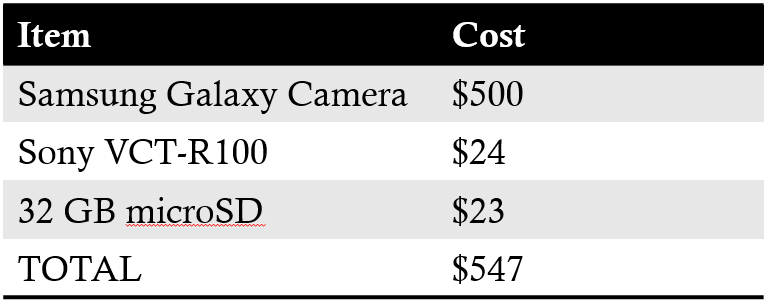
\includegraphics[scale=0.5]{images/budget.png} \\
		
		I chose the Sony VCT-R100 because it is small, compact, and durable. While there are cheaper options available I wanted the tripod to last long enough to be worth the purchase.
		I chose the 32GB microSD card because we want a memory card that is large enough to hold all of the photos taken during a lecture so that if for some reason the transfer of photos to thee analysis server fails partway through the lecture, the images won't be lost.
		The choice of the Samsung Galaxy Camera was pretty easy at this point since we've been agreed on our camera choice for months now.
	
	% 18th Entry
	\section{Individual Work Exploring more OpenCV filters 11/15/2012}	
	
	I spent several hours experimenting with various filters to try to get a pure white background with pure black writing on the board. I found that my best results
	came when I used a combination of filters. I first converted the image to greyscale. After this i used the cv.Threshhold function on it twice to filter out imperfections in the background, and used cv.Erode to further emphasize the text. The following image was the best I was able to achieve with filters: \\
	
		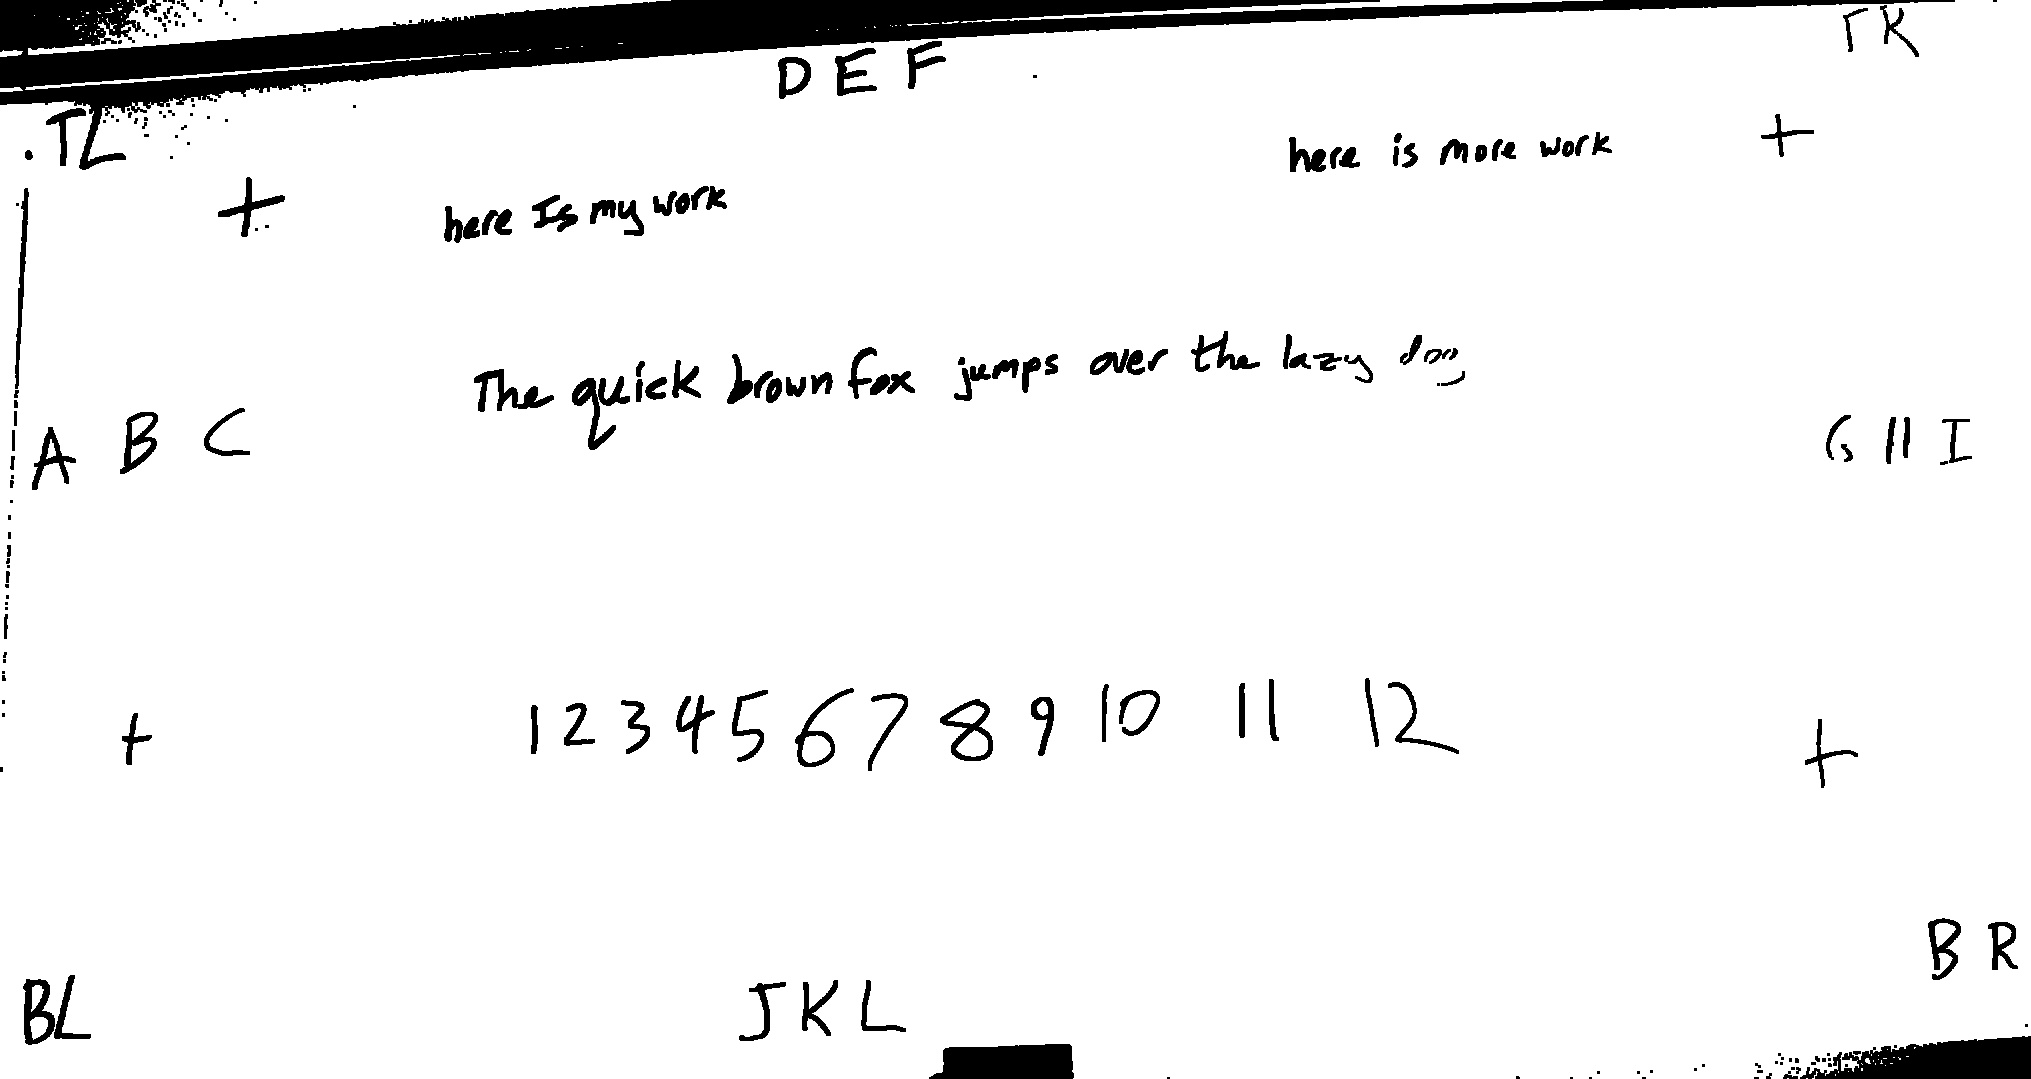
\includegraphics[scale=0.2]{images/bestResult.jpg} \\
	
	As you can see there are still issues with the image, but overall it turned out quite well. The elements key to this image's successful conversion were the threshold values chosen for the cv.Threshold section. This is a key weakness for this type of image processing because it required very precise numbers and I currently don't know how to generate the right numbers automatically. Instead i had to guess and check a bit. This means that attempting to run the same code on a different image would likely result in poor image quality.

	Another success I had was in creating a program to detect the edges of a writing in a photograph. It uses a combination of the cv2.GaussianBlur filter and cv2.Canny to detect where the edges are and highlight them in white. after this i set everything else black. Inverting this creates a white image with black outlines of white text. After this i used cv.Erode in an attampt to fill in the outlines so that they looked like black text. Unfortunately, this also detracted from the image's writing clarity as the blacks tended to blur together. I'm currently looking for some method to fill in the inside of the black outlines without eroding outwards as well. The following are the three image results from the three steps: \\
		
		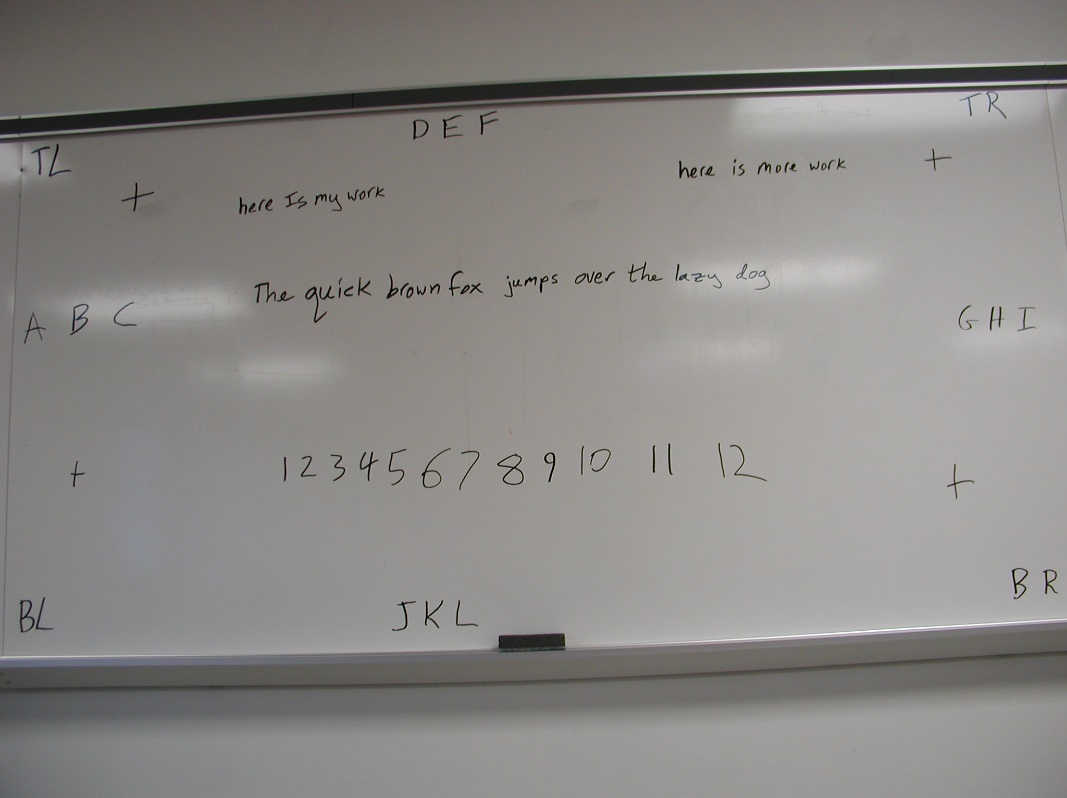
\includegraphics[scale=0.27]{images/cannyOriginal.jpg}
		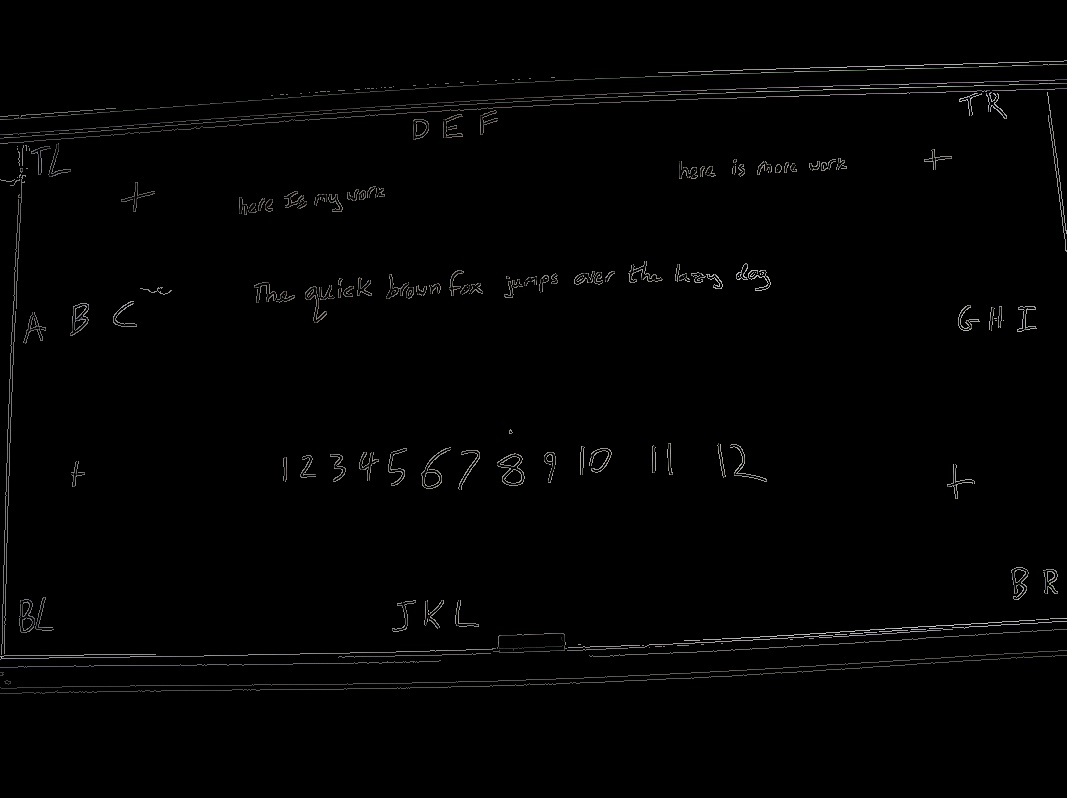
\includegraphics[scale=0.2]{images/cannydemo.jpg} \\
		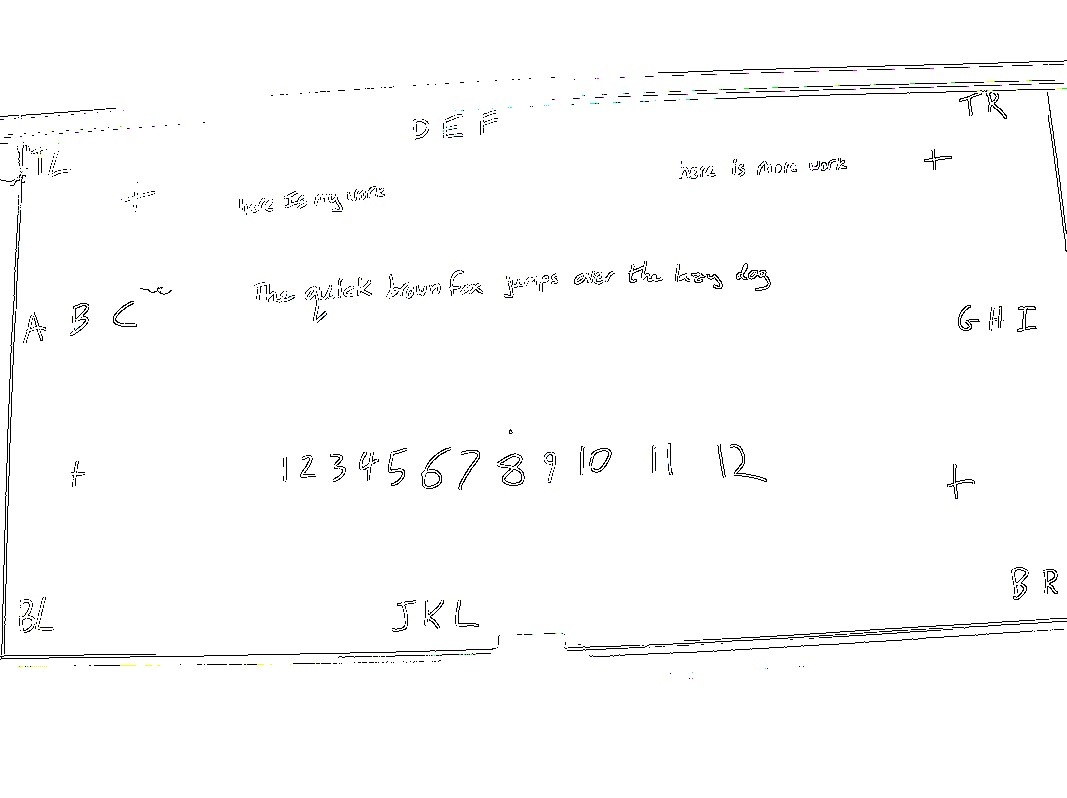
\includegraphics[scale=0.2]{images/cannydemo2.jpg}
		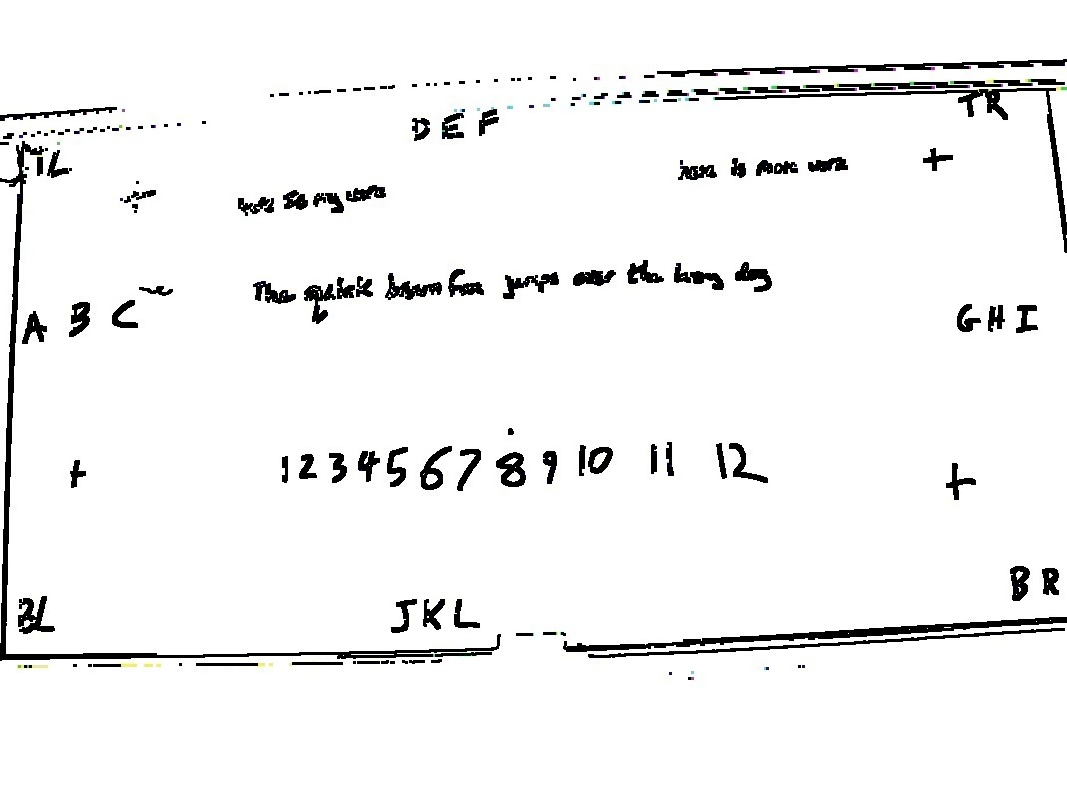
\includegraphics[scale=0.2]{images/cannydemo3.jpg} \\

	% 17th Entry
	\section{Individual work creating a standard set of images for our image processing tests 11/12/2012}

	Creating these images actually took a lot more work than I originally expected. Not because they were difficult to photograph, but because obtaining a tripod and finding an empty room in Breakiron took work. The library was out of loaner tripods so i ended up contacting one of my bosses, who happened to know another staff member who had a tripod lying around that i could borrow.\\
	I then returned to Breakiron only to find that all the classrooms were occupied. I ended up having to leave, and came back a few hours later to take my pictures.\\
	
	My test set of photos were of the following: an image of a blank whiteboard,  an image of the whiteboard full of handwriting, and several images of me blocking different sections of the whiteboard. An interesting side effect of this endeavor is that clothing can really effect how Colin's current image processing software works. I was wearing a gray shirt with black horizontal stripes, and his software had a great deal of trouble differentiating my shirt from my actual handwriting.\\
	
	% 16th Entry
	\section{Individual Work Researching OpenCV 11/5/2012 - 11/7/2012}
		\subsection{Installation}
			Spent a few hours installing and familiarizing myself with OpenCV-Python. It is an add-on library written in C that can be used with Python and C++.
		\subsection{Image Filtering Overview}
		There were three filters that i found to be especially useful in OpenCV.
			\begin{itemize}
				\item Laplace
				\item Erode
				\item Dilate
			\end{itemize}
		\subsection{Laplace}

			The Laplace filter basically makes all black pixels go white and all white pixels go black. This is useful because it ignores the colored pixels and gives nice readable results. \\

			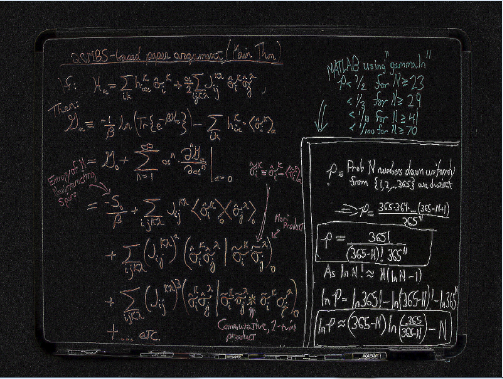
\includegraphics{images/laplaceSmall.png} \\
		
		\subsection{Erode}

			Erode could be very useful because it makes writing on the whiteboards thicker and more legible. this could be useful in cases where the writing is too thin to see/easily read after other filters have been applied.\\

			Original:\\
			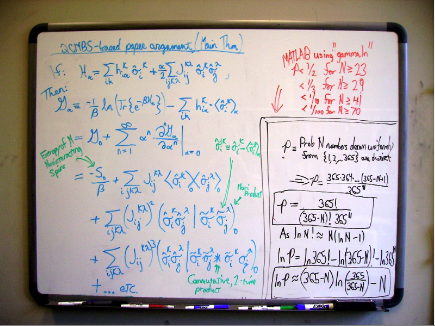
\includegraphics{images/originalSmall.png} \\
			Erode1:\\
			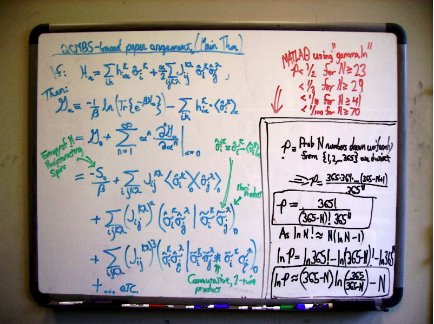
\includegraphics{images/erodeSmall1.png} \\
			Erode2:\\
			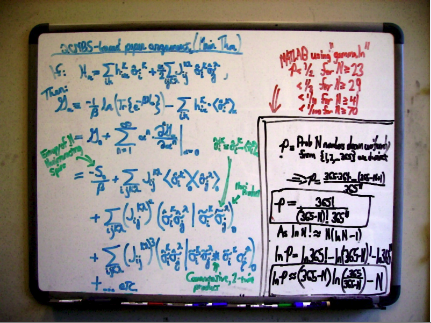
\includegraphics{images/erodeSmall2.png} \\
		
		\subsection{Dilate}
			The Dilate filter makes everything lighter, as seen below:\\

			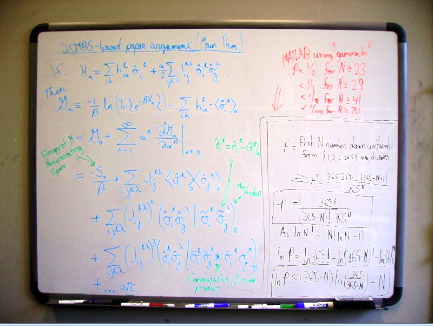
\includegraphics{images/dilateSmall.png} \\

	
	% 15th Entry
	\section{Individual work creating Minutes for Post Panel 2 10/31/2012}
	
		\noindent Meeting Minutes for Post Panel 2 (10/31/2012):
		
		\subsection{Members Present}
			Robert Midkiff, Griffin Dunn, Colin Madigan, Phil Stahlfeld
		\subsection{8:00 to 8:15 Panel 2 Review}
			\noindent Reviewed Material Covered in Panel 2
			\begin{itemize}
					\item Showed progress with Python filters
					\item Discussed success applying filters to specific cells in images.
					\item Discussed progress with image filtering tech. in general.
					\item Discussed attempts to contact Microsoft for their sourcecode.
			\end{itemize}
			
		\subsection{8:15 to 8:25 Future Progress}
		
				\begin{itemize}
					\item Discussed gantt chart
					\item Discussed future goals for ProPANE
					\item Asked for feedback and suggestions for current work.
						\subitem{Dr. Midkiff was pleased with our progress and told us to keep up the good work}
					\item Summarized what we need to do before next panel
				\end{itemize}
			
		\subsection{8:25 to 8:30 Wrap Up}
			
				\begin{itemize}
					\item Discussed Hurricane Sandy
					\item Wrapped up discussion and thanked Dr. Midkiff for coming.
				\end{itemize}
	
	% 14th Entry
	\section{Individual work creating Minutes for Panel 2 10/29/2012}
	
			\subsection{Members Present}
				Professor Watkins, Professor Thompson,, CTDI team, Griffin Dunn, Colin Madigan, Phil Stahlfeld
			\subsection{15:00 to 15:05 Review}
				
				Reviewed Documentation and Technical Specifications \\
				
			\subsection{15:05 to 15:15 Discussed Completed Work}
				
				\subsection{Image Processing}
					\begin{itemize}
						\item Showed progress with Python filters
						\item Discussed ideal image quality
							\subitem{Used CamScanner as ideal to strive for}
						\item Showed progress with ImageJ filters
						\item Discussed attempts to ob
					\end{itemize}
				
				\subsection{Sourcecode}
					\begin{itemize}
						\item Showed that ImageJ could be useful because it is open source. \\
						\item Discussed attempts at obtaining CamScanner source code. Concluded that it would be too difficult to find useable code through java decompiling. \\
						\item Prof. Thompson suggested that if Microsoft does not respond to our email soon we should talk to both him and Prof. Watkins so that they can try their contacts within Microsoft. \\
					\end{itemize}
				
			\subsection{15:15 to 15:25 Discussed Future Plans}
				
				\subsection*{Discussed Gantt Chart}
					\begin{itemize}
						\item Prof Thompson suggested that we allocate more time for tasks that could be more difficult.
						\item ProPANE was asked if they had looked into OpenCV along side Python and Java filters. 
							\subitem{No, but it is scheduled into our workflow}
						\item Discussed how we planned to come up with a final plan
							\subitem{By trying many approaches and choosing those that show that they can effectively meet our goals}
					\end{itemize}
				
			
			\subsection*{15:25 to 15:30 Wrap Up Questions}
				
				ProPANE showed that they could 'speak in full sentences' and that they were on the right track.
	
	% 13th Entry
	\section{Group Work Preparing For Panel 2 10/24/2012}
		\begin{itemize}
			\item Began creating presentation document for Panel 2
				\subitem{This document was then discarded as we came up with a new structure for the document}
			\item Created powerpoint of our current work on image processing.
			\item Worked a little with colin on Gannt Chart
			\item Developed gameplan with group on what we'd do for Panel 2
		\end{itemize}
			
	% 12th Entry
	\section{Individual Work Collecting Whiteboard images with various cameras 10/22/12}
		\subsection{Purpose}
		Today I worked to collect several images of whiteboards using different cameras. The purpose of this exercise was to gain a better understanding of what is needed from our image capture device. Analyzing the results of a range of devices we hope to better understand what the limiting factors are with indoor image capturing. \\
		\subsection{Setup}
		I captured images from two main locations: On a table in front of the whiteboard and on top of the projector. I decided to add images from near the projector just in case the table is too close to the whiteboard.
		Note that the Whiteboard was 8 feet wide for all of these images.
		
		The following images were taken 9 feet away from the whiteboard with a 3.3 Megapixel Olympus C-3040ZOOM: \\
		
		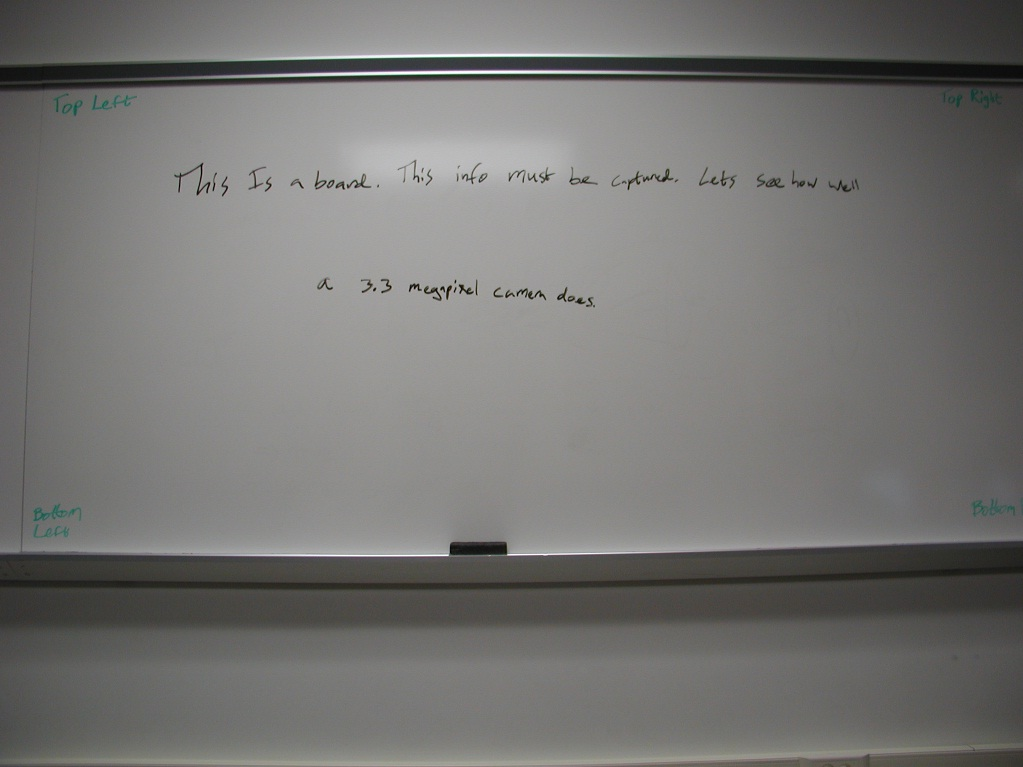
\includegraphics{images/UnmodifiedClose.jpg} \\
		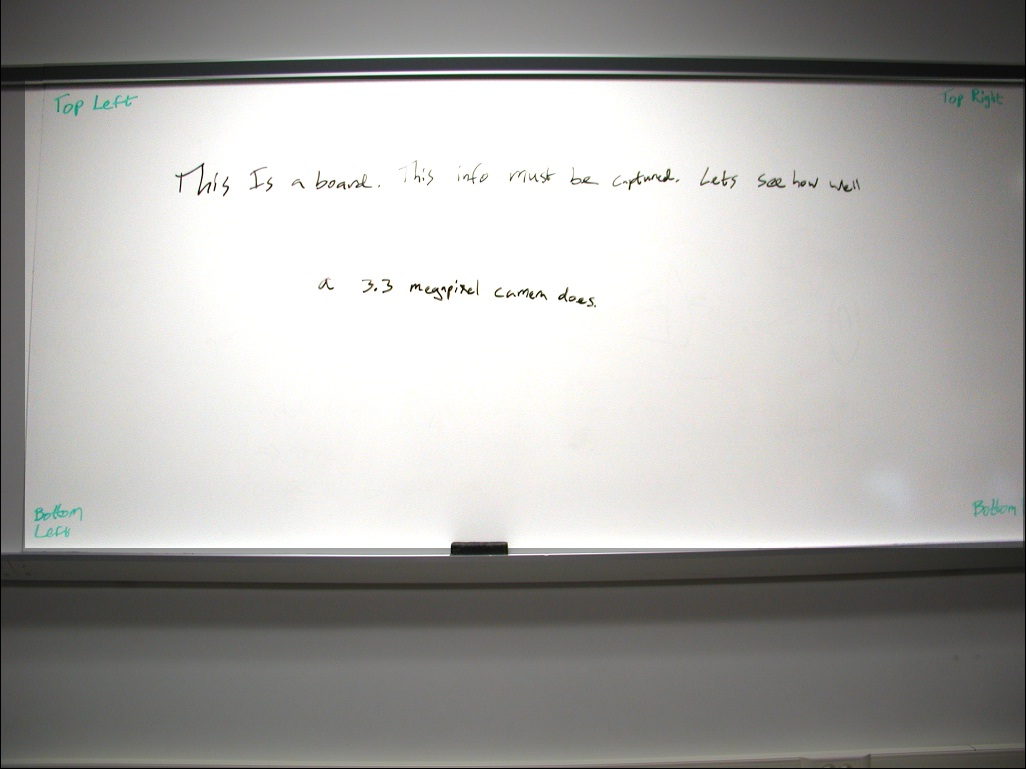
\includegraphics{images/ModifiedClose.jpg} \\
		
		The following images were taken while 9 feet away from the whiteboard with the HTC Inspire's 8 Megapixel camera: 
		
		\includegraphics{images/UnmodifiedPhoneClose.jpg} \\
		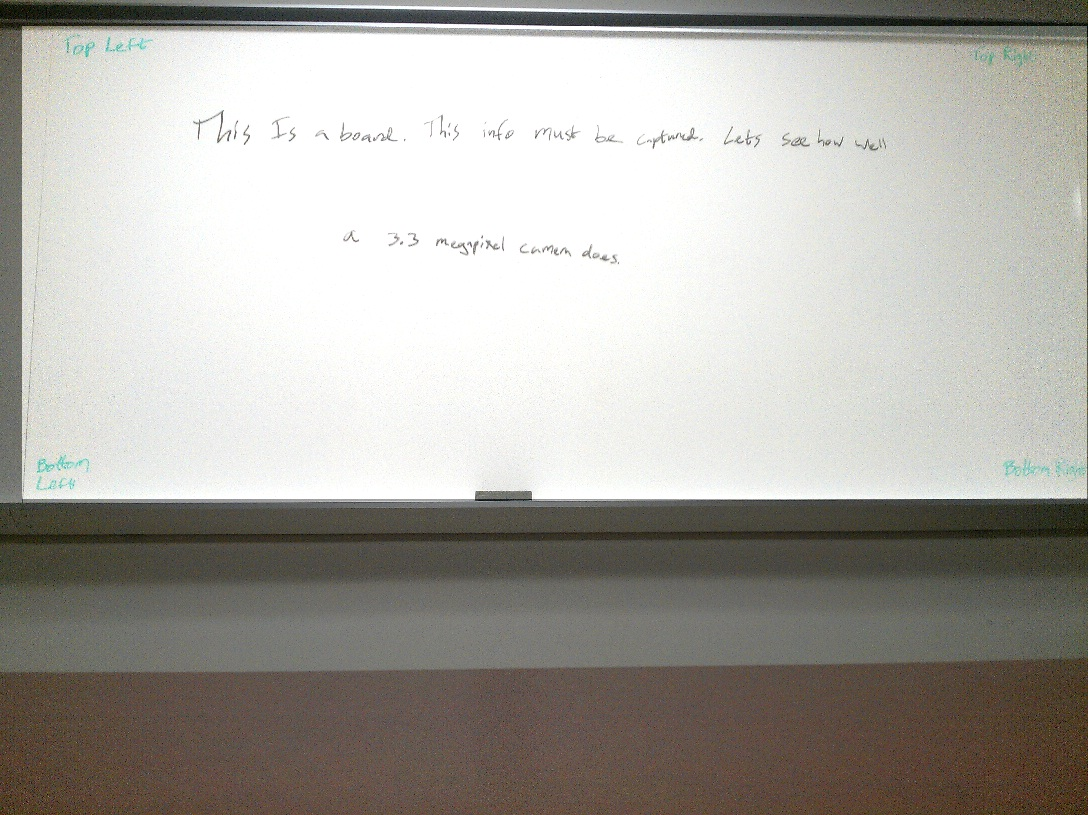
\includegraphics{images/ModifiedPhoneClose.jpg} \\
		
		The following images were taken while 7.5 feet away from the whiteboard with a 12.1 Megapixel canon powershot sd1300:
		
		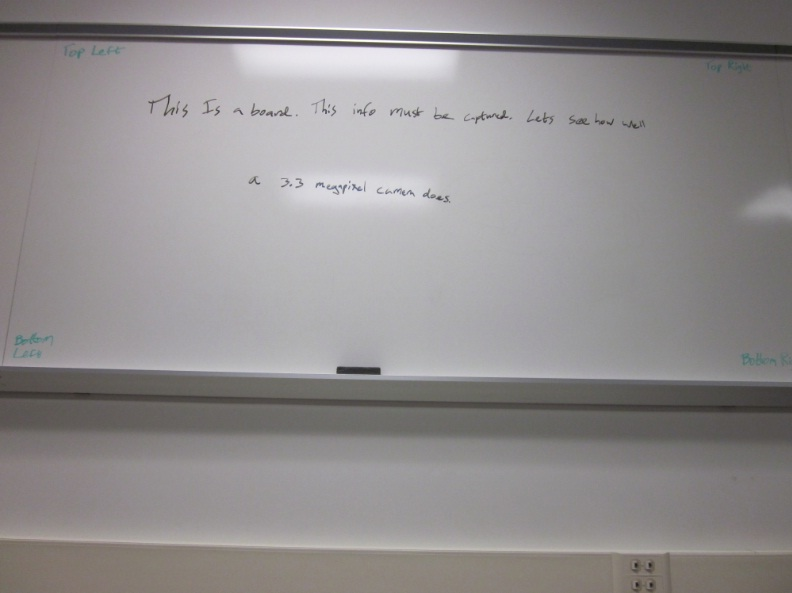
\includegraphics{images/TableLevelCanon.jpg} \\
		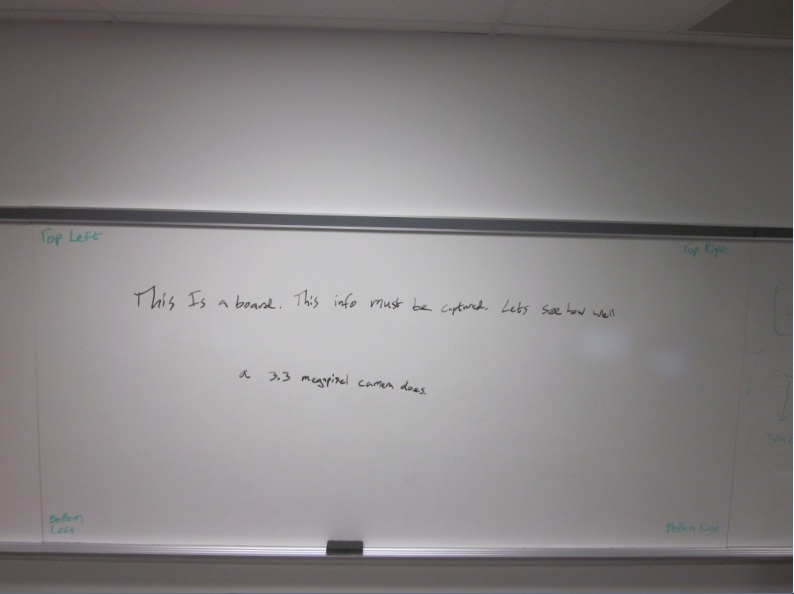
\includegraphics{images/ProjectorHeightCanon.jpg} \\
		Notice how much less glare there is from the lights when the camera is at projector height. This will make removing background noise much easier. Not only that, the highter vantage point would likely capture more of the bord and less of the professor.\\
		
		\subsection{Conclusion}
			Note that all modified images were modified using ImageJ, the open source image editor i found that uses java
			The 3.3 MP camera and my 8MP camera both required about 9 feet distance from the board minimum, while the newer canon powershot sd1300 only required about 7.5 feet distance from the board.\\
			
			Something that isn't as immediately obvious, but is more noticable when looking at the fullsize images, is the fact that the higher megapixel cameras did a better job capturing information because zooming in allowed for crisper, clearer letters. \\
		
	% 11th Entry
	\section{Individual Work on Sourcecode 10/20/1023}
		
		\subsection{CanScanner Sourcecode}
		I viewed CamScanner's sourcecode by following the instructions on this forum: \\
		http://stackoverflow.com/questions/3593420/android-getting-source-code-from-an-apk-file\\
		
		\begin{itemize}
			\item Download .apk
			\item Rename remove .apk ending from name and put .zip in it's place
			\item Extract all files
			\item Download dex2jar
			\item Run dex2jar on the classes.dex file found in CamScanner's extracted files
			\item Run java decompiler on the classes.dex.dex2jar file created in step 5
			\item Save all class files
		\end{itemize}
		
		After attempting to understand CamScanner's code for 1.5 hrs, I decided that the code wasn't readable enough to use in our project. It might have useful information in it somewhere, but the decompiled naming scheme, lables, etc weren't readable enough for easy analysis. Will go back to this sourcecode if other options fail.
		
		\subsection{Alternative Program}
		
		I found an opensource program called ImageJ. This program has features similar to CamScanner's image filtering options...though they don't work as well. By adjusting the brightness and contrast of an image i was able to greatly enhance text's clarity: \\
		
		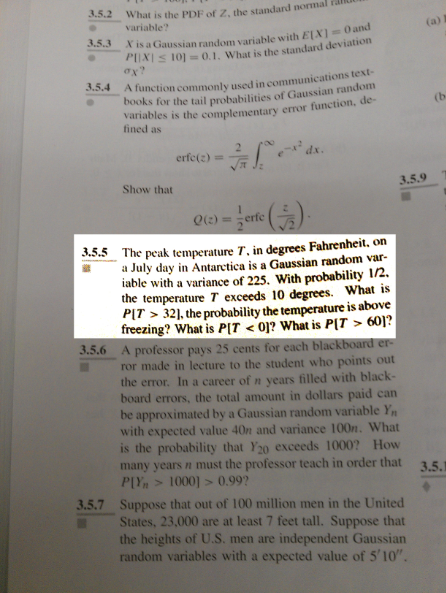
\includegraphics{images/ImageClarityWithImageJ.jpg} \\
		
		I think that this program could be useful if we decide that we want to write an image enhancement progarm in java or if we want to include some enhancement features in an android app. \\
		
		\subsection{Python Libraries}
		
		I briefly looked into different options we had in python and found two libraries that looked like they might be useful for image enhancement: \\
		
		The ImageFilter module has many pre-defined enhancement filters for the 'filter' method. \\
		http://www.pythonware.com/library/pil/handbook/introduction.htm\\
		
		Advanced enhancement features can be found in the ImageEnhance module. \\
		http://www.pythonware.com/library/pil/handbook/imageenhance.htm \\
	
	
	% Tenth Entry
	\section {Risk Meeting, Future Tasks 10/18/2012}
		\subsection{ProPANE and Prof. Thompson Meeting}
		We met with Prof. Thompson today to discuss our risk analysis. He gave us a better understanding of what he expects from us going forward in the semester.  The goal is not to complete most every aspect of our project. Instead, he wants us to try out lots of different way to impliment various aspects of the project, and from this experimentation be able to say definitively which strategy we are going to employ and why we want to use it. \\
	
	
	% Ninth Entry
	\section{Website updating and Language Editing 10/12/2012}

		\subsection{Language Editing}	
	Went through documentation checking for grammar. Apparently I missed quite a bit when it came to spelling mistakes. Will look at .tex documents with spellcheck enabled from now on. \\
	
		\subsection{Website Updating}
	Updated Team Member page of our website. It now has the following blurbs next to each picture: \\
	
	Griffin: \\
	Griffin is a senior computer engineering and management double major at Bucknell University. He is the Service Chair for the Bucknell IEEE Student chapter and an active participant in Delta Upsilon Fraternaty. Over the summer he worked at the Computer Center at Bucknell University as an Enterpise Systems Developer, developing web pages for clients throughout the university. \\
	
	Colin: \\
	Colin is a senior electrical engineering major at Bucknell University. He is a member of Tau Beta Pi, the Honors fraternity on Bucknell campus and he is a member of the Bucknell IEEE student chapter. Over the summer he Interned for Blue Belt Technologies, a company that specializes in intelligent orthopedic surgical instrumentation.\\
	
	Phil: \\
	Phil is a senior computer engineering major at Bucknell University. He is president of Tau Beta Pi, the Honors fraternity on Bucknell campus and is a member of the Bucknell University  IEEE student chapter. Over the summer he Interned for Northrop Grumman, Space division of electronic systems on automated bench marking of high performance computers. \\
	
	% Eigth Entry
	\section{Classwork on Brainstorming, etc 10/11/2012}
		\subsection{Stages in the Feasibility Stage}
			There are 5 stages in the next  portion of our development process:
			\begin{itemize}
				\item Stage 1: Brainstrom
				\item Stage 2: Identify Risk
				\item Stage 3: Prioritize Risks
				\item Stage 4: Develop Deliverables for each Risk
				\item Stage 5: Divide and Schedule work
			\end{itemize}
			
			\subsection{Brainstorming}
			There are three major sections to our project:
				\begin{itemize}
					\item Capturing
					\begin{itemize}
						\item All tasks related to capturing all information written on the whiteboard
					\end{itemize}
					\item Sending
					\begin{itemize}
						\item All tasks related to sending and recieving information between devices
					\end{itemize}
					\item Processing
					\begin{itemize}
						\item All tasks related to processing the images once they are recieved by the linux machine
					\end{itemize}
				\end{itemize}
			
			\emph{Capturing} 
			\begin{itemize}
				\item Decide on a camera
				\item Designing/purchasing a stand
				\item Figure out setup stuff
				\item Determin min/max distance from board based on camera lense and number of megapixels
				\item Look into rooting camera (maybe. depends if it can install apps that aren't in the app store)
				\item Look into making image capturing process automated
				\item look into designing android app
				\item how to take periodic images
				\item how to communicate with camera using button or sensor
				\item adjust shutter speed and/or ISO to accomodate different light levels. (automatic with flash disabled)
			\end{itemize} 
			
			\emph{Sending}
			\begin{itemize}
				\item Look into communication between android and linux
				\item Ways to store/send images
				\item Ways to make sending info reliable
				\item How to send data automatically
				\item How to recieve data on linux
				\item How to automate linux processes
				\item How to send to/connect to moodle folder.
			\end{itemize}
			
			\emph{Processing}
			\begin{itemize}
				\item How to remove background noise
				\item how to stitch in information covered by professor
				\item how to change brightness/contrast
				\item look into better ways of processing images
				\item look into what image processing libraries are available
				\item maybe look into what programs are available to do these sorts of things for us.
				\item look into ways to automate actions performed by random programs
				\item look into ways to do what we want with premade programs and just automate the processes somehow
				\item What sorts of processing technologies are available to us?
			\end{itemize}
			
		\subsection{Identify Risks}
		There are are 3 main areas that represent the highest risks to our project:
			\begin{itemize}
				\item Image Proessing on the linux system
				\begin{itemize}
					\item Everything associated with it. How will we do this???
				\end{itemize}
				\item Deciding on Camera
				\begin{itemize}
					\item This will define how we will research the image captureing process. There isn't very much that we can do on the capturing side of things before this decision is made.
				\end{itemize}
				\item Look into how to use camera using application
				\begin{itemize}
					\item The creation of an application that will automate the image capturing process on the android camera
				\end{itemize}
			\end{itemize}
		\subsection{Deliverables}
			\emph{Deliverables for Processing:}
			\begin{itemize}
				\item Demo code that removes noise
				\item Demo code identifying professor on image
				\item Demo code removing professor from image
				\item Demo code splicing prof-free images together
				\item Demo code auto-grabbing new images + removing prof, splicing together, etc.
				\item Demo code of auto-everything
			\end{itemize}
			\emph{Deliverables for Capturing}
			\begin{itemize}
				\item Demo image taken by android camera by our own app
				\item Demo android camera taking pictures automatically every few seconds
				\item Demo app setup process such that it can be left to auto=take pictures all period
				\item Demo app sending photos to linux machine
				\item Auto=focus
				\item Manual Zoom during setup.
			\end{itemize}
		
	% Seventh Entry
	\section{Group Work With Colin To Finish Up Documentation 10/10/2012}
		\noindent \emph{Electronic Whiteboards-} \\
Smartboards are full sized, touch sensitive whiteboards. You can project images onto them with a projector and then make edits/additions to them with any pointed object. The touch sensitive board senses where you are writing on the board and adds electronic corrections to the image/document. These devices do not compete as directly with our project as the smartphone apps and the scanners because they are not nearly as portable. They are the size of a standard whiteboard and thus cannot be easily moved between classrooms.
            \begin{itemize}
                \item SMART Board
                \item Panasonic's Panaboard
                \item Hitachi's Starboard
                \item The Promethean Board
            \end{itemize}
			

			\subsection{Introduction}
The following paragraphs are descriptions of several smartphone apps that contain features wish to emulate in our own project. They in many ways solve the needs of our current clients. We therefore hope to take some of these phone-app features and modify them to better meet the needs of our own clients. \\
				\subsection*{Whiteboard Capture Pro}
Source: Beetlebug Software's website\\
{\color{red} \url{http://www.beetlebugsoftware.com/}} \\
					
This is an iPhone app that takes a picture of a white board and then analyzes it for key content. The user selects objects to remove from the photograph. This leaves only the writing on the board behind. The App then analyzes the writing and removes the background image of the whiteboard itself. This sometimes leaves fuzz or imperfections in the white background, so there is then a slider available to filter out this extra noise/fuzz that shows up in the end product. The resulting image is a pure white background with handwriting on it.These photos can then be saved, cropped, shared, and organized within-app tools. \\
				\subsection*{WBConference}
Source: Elecom'e website\\
{\color{red} \url{http://app.elecom.co.jp/en/wbcap/ios/manual.html}} \\
					
This is an Android app that competes with our product because it is another whiteboard capturing device. WBConference differs from Whiteboard Capture Pro in that it is able to automatically recognize which sections of the board are whiteboard. This then allows it to apply its ìmagnified keystone correctionî to remove the excess background imagery. In cases that it cannot recognize the board you can zoom in on just the board boundaries manually before capturing the image. The app has contrast adjustment and image rotation as well so you can take images from any orientation without problems.This app has editing features as well so you can add postscripts or speech bubbles to the images. The files can then be saved as PDFs along with any notes you want to add to them.This app has a widget for the home screen for quick image capturing, and you can set up an email address for quick delivery of the images to an external source. \\
				\subsection{CamScanner -Phone PDF Creator}
Source: Intsig's Website
{\color{red} \url{http://www.intsig.com/en/camscanner.html}} \\
					
This is the most downloaded ëscannerí app on the market. With it you can take photos of any document, whiteboard, etc that you want. You then go through an editing process in which you can select the important portion of the photograph, change the detail level, contrast, light/darkness etc. It will then save your new document in any number of saved folders. You can make notes about each image and these notes will be saved with the image. You can email, print, fax, or transfer via Bluetooth any of the photos. You can also upload your images to google docs, evernote, skydrive, dropbox, or box.net. These documents get saved as PDFs. There are different enhancement modes: No enhance, low and high enhance, gray mode, and B\&W Document modes. These different modes will be better depending on the environment or object that youíre trying to scan. The B\&W mode is particularly helpful when scanning books/papers because it does a better job of removing the background noise. This app allows for batch photo taking and batch photo scanning, so you can take multiple pictures and it will scan them all at the same time. \\
				\subsection{Whiteboard Capture Pro}
Source: Magnicode's website\\
{\color{red} \url{http://www.magnicode.com/}} \\
					
This app is a dumbed down version of the previous three. It does the job, it scans and enhances images, it just isnít as well known as the others and thus doesnít have the money/time to invest in extra features. This aside, it does work, it is free, and it does save images as PDFs for later use. You can email these photos to yourself and store them in different photos. You can attach notes to your images and you can enhance the quality of the whiteboard picture with their auto-enhance tool. On the upside, it IS a much smaller program than your avg whiteboard capture app. Over all a smaller lighter free alternative. I installed this app on my phone and I had trouble using it because it kept crashing. \\

     \subsection*{Conclusion}
These smart phone apps will be some of the greatest competition to our project because they meet many of our client's needs already. Not only that, they're free applications so our clients wouldnt need to spend money either. The following is a list of features that we should attempt to emulate when designing our own product.

All of these applications contain ways to filter out background noise so that whiteboards appear pure white and text looks crisp and clean. This will be an important aspect of our own product because our image capture device will be subject to a wide variety of lighting situations and will need to be able to adapt to any of them.
Another key feature is the ability of these apps to save and send the images via email, google docs, and other online mediums. This will be an important point in our project as well.
Another good feature was the ability for some of the apps (CamScanner for example) to correct for image angles. If the board is photographed from an angle, the smartphone apps will compensate so that the final scanned image looks like it was taken straight on. \\

        \emph{Desirable features not found in smartphone apps:}
        \begin{itemize} \itemsep -2pt
            \item Photo splicing: These apps do not combine images to add in details covered by professor's body.
            \item Automatic: These apps do not automatically capture images, process them, and then send them away. They instead require user feedback every step of the way.
        \end{itemize}

By adding these features to the functionality currently found in modern apps we hope to create value for our customer.


	 \subsection*{Cameras we could use in our project}
Here are the current top three cameras that we think could help us the most when building our image capturing system.

\begin{itemize}
    \item Nikon COOLPIX S800c 16 MP Digital Camera
    \begin{itemize}
        \item \url{http://www.amazon.com/Nikon-COOLPIX-Digital-Optical-3-5-inch/dp/B0090SLKUM}
    \end{itemize}
    \item Samsung Camera EK-GC100 Galaxy Camera
    \begin{itemize}
        \item \url{http://pdadb.net/index.php?m=specs&id=3813&c=samsung_ek-gc100_galaxy_camera}
    \end{itemize}
    \item Polaroid SC1630 Smart Camera
    \begin{itemize}
        \item \url{http://www.upi.com/Science_News/2012/01/16/Polaroid-joins-digital-camera-arena/UPI-61851326750025/}
    \end{itemize}
\end{itemize}

We are interested in them because they are cameras running the Android operating system. This means that we could create our own custom application for these devices, greatly simplifying our design process. These cameras would also be useful because they can connect to Bucknell's wifi network. This would allow us to wirelessly transferr information from the cameras to whatever image processing hardware we decide to connect it to. The main drawbacks at the moment with these Android cameras is that two of them haven't been released yet (Samsung and Polaroid). IF they are released in time, they would be the most desireable of the various camera options available.

\subsection*{Details on Learning Disabilaties}
        \subsubsection*{Introduction}
One of the major motivating factors behind designing our image capturing system is to help meet the needs of students with disabilities. The term "students with disabilities" is a very broad term, however, so we would like to use the following section to help discribe some of the things that mildly disabled students have trouble with at Bucknell, and would therefore need our system to capture information presented on the board for them.
\\
Source: \\
{\color{red} \url{http://www.sfasu.edu/disabilityservices/facultyandstaff/for_service_providers/note_q_a.asp}} \\
\\
Disabilities that students might have that impair their ability to take notes:
    \begin{itemize}
        \item Visual Impairments
        \begin{itemize}
            \item May be fully blind and need notes translated into Braille
            \item May not see well and need large print letters
            \item May have trouble copying information from whiteboards, projectors, etc.
            \item May have trouble seeing certain colors when framed by a white or black background
        \end{itemize}
        \item Specific Learning Disabilities
        \begin{itemize}
            \item Reading Disability
            \item Writing Disability
            \item Spelling Disability
            \item Inability to copy what they see
            \item Inability to write what they hear
            \item Inability to write legibly
            \item Number Reversal problems
        \end{itemize}
        \item Mobility Impairments
        \begin{itemize}
            \item Physically unable to write
            \item Physically unable to write quickly
            \item May be unable to effectively handle a writing impliment
        \end{itemize}
        \item Partial or Full loss of hearing
    \end{itemize}

This is just a small portion of the many disabilities faced by students in universities around the world. We hope to help them by giving them full access all information presented on boards during lectures. By providing easily accessible, easily modifiable images, we hope to help even the playing field for students with disabilites.
Secondary goals of our project will help to make the learning process even easier. Some students get distracted if they see more than one line of text at a time. If we have enough time we will help these students by providing slide bars that will cover portions of the images that students are not currently viewing. This and many other minor features are things that we will accomplish if we have free time after completing our primary objectives.








	% Eigth Entry
	\section{Notes from Client meeting 10/05/2012}
	Point to git repository on website or it 'never happened.' The only things Thompson knows about are those found on the website.
	
	How image processing is generally don
	Types of image processing
	
	\emph{Important points given during meeting:}
		\begin{itemize}
			\item Wireless
			\item Way to tell system that "this" is a key fram/moment.
			\begin{itemize}
				\item Instructor marked key moments/frames with a button or gesture or something.
			\end{itemize}
			\item Generate list of 'it would be nice if...'
			\item Email about sitelines, optimal viewing angles, aspect ratios, etc.
			\item Re-organize Related Technologies
			\item Want: What are we DOING with all information presented in research/documentation
			\item Want: Paragraph at end of smartphone app summaries, synthasizing/analyzing information presented in summaries
			\item Microsoft: This project was very close to what we are going to do, that is why we are going into so much depth on it.
			\item Give information on the whole field of Image processing.
			\item Give information about students with various disabilities that would benefit from our product
			\begin{itemize}
				\item 'This is what the students need and why'
			\end{itemize}
		\end{itemize}
	\emph{Notes on stuff we'll be doing next:}
		\begin{itemize}
			\item Figure out what you're doing in the next couple months
			\item Look at what tasks you could be doing, analyze the risk of each task.
			\item Arrange everything by risk. Highest risk on top!
			\item Assign people reduce the risks of each task
			\begin{itemize}
				\item You can have multiple people working on a single thing. The idea is to reduce the high risk tasks asap so that they don't kill the project later on.
			\end{itemize}
			\item Assign 3-4 deliverable items to each person to reduce risk
			\item Can have multiple people per task
			\item Throw resources at the rediculously risky to get it done, else project fails
		\end{itemize}
	% Seventh Entry
	\section{Group work on Memo 10/03/2012}
		Worked with Colin and Phil to create the memo for our 10/05/12 meeting.


	% Sixth Entry
	\section{Individual Work on Further Research on Phone Apps 09/20/2012}
	
		\subsection{APPS}
		I was looking into android cameras earlier and found two possible candidates. One of them (The Nikon) has been released already, but the Samsung looks like a much better product if we can get it in time.
		
		Nikon COOLPIX S800c 16 MP Digital Camera\\
		Samsung Camera EK-GC100 Galaxy Camera\\
	
			
		\subsection{Whiteboard Capture Pro}
		
			This is an iPhone app that takes a picture of a white board and then analyzes it for key content. The user selects objects to remove from the photograph. This leaves only the writing on the board behind.\\
			
			The App then analyzes the writing and removes the background image of the whiteboard itself. This sometimes leaves fuzz or imperfections in the white background, so there is then a slider available to filter out this extra noise/fuzz that shows up in the end product. The resulting image is a pure white background with handwriting on it. These photos can then be saved, cropped, shared, and organized within-app tools.\\
			
			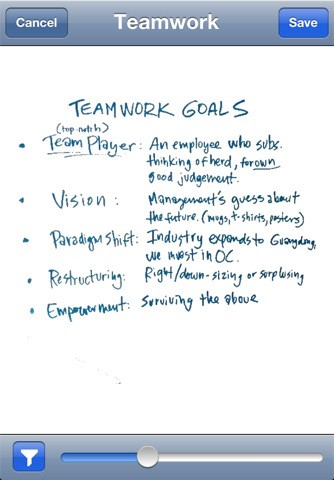
\includegraphics{images/team1.jpg}
			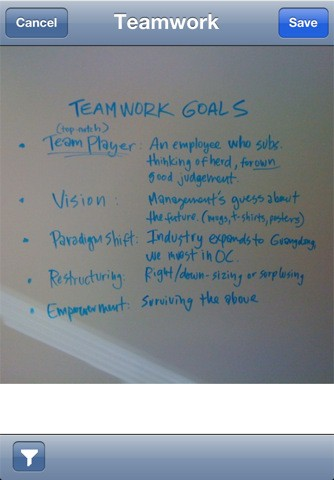
\includegraphics{images/team2.jpg}
			
			Notice the slider at the bottom of the image on the left. This is the contrast slider that helps remove background noise.

			(guesswork)
			Contrast sliders work by analyzing the transition colors between the white and the eventual blue of the writing. The higher the contrast, the faster the transition must be between pure white and pure blue. If the transition is too slow, the transition pixels are assumed to be noise and removed from the photo. This is useful both in making the handwriting appear crisp and in removing random background smudges. Smudges are of course removed because they don’t have the crisp transition periods found in the writing on the board.
			(Now back to research)
			
		\subsection{WBConference}
			This is an Android app that competes with our product because it is another whiteboard capturing device. WBConference differs from Whiteboard Capture Pro in that it is able to automatically recognize which sections of the board are whiteboard. This then allows it to apply its “magnified keystone correction” to remove the excess background imagery. In cases that it cannot recognize the board you can zoom in on just the board boundaries manually before capturing the image. The app has contrast adjustment and image rotation as well so you can take images from any orientation without problems.\\
			
			This app has editing features as well so you can add postscripts or speech bubbles to the images. The files can then be saved as PDFs along with any notes you want to add to them. This app has a widget for the home screen for quick image capturing, and you can set up an email address for quick delivery of the images to an external source.\\

		\subsection{CamScanner -Phone PDF Creator}
			This is the most downloaded 'scanner' app on the market.\\
			
			With it you can take photos of any document, whiteboard, etc that you want. You then go through an editing process in which you can select the important portion of the photograph, change the detail level, contrast, light/darkness etc. It will then save your new document in any number of saved folders. You can make notes about each image and these notes will be saved with the image. You can email, print, fax, or transfer via Bluetooth any of the photos. You can also upload your images to google docs, evernote, skydrive, dropbox, or box.net. \\
			
			These documents get saved as PDFs.\\
			
			There are different enhancement modes: No enhance, low and high enhance, gray mode, and BandW Document modes. These different modes will be better depending on the environment or object that you’re trying to scan. The BandW mode is particularly helpful when scanning books/papers because it does a better job of removing the background noise. \\
			
			CamScanner allows for batch photo taking and batch photo scanning, so you can take multiple pictures and it will scan them all at the same time.\\
			
			You can password protect your documents and even save different document sizes.\\
			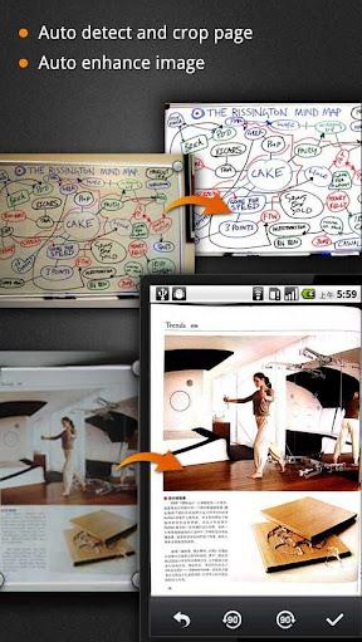
\includegraphics{images/autoCrop.jpg}	

		\subsection{Whiteboard Snap}
		
		This app is a dumbed down version of the previous three. It does the job, it scans and enhances images, it just isn’t as well known as the others and thus doesn’t have the money/time to invest in extra features.\\
		
		This aside, it does work, it is free, and it does save images as PDFs for later use. You can email these photos to yourself and store them in different photos. You can attach notes to your images and you can enhance the quality of the whiteboard picture with their auto-enhance tool.\\
		On the upside, it IS a much smaller program than your avg whiteboard capture app. Over all a smaller lighter free alternative.\\
		I installed this app on my phone and I had trouble using it because it kept crashing.\\

	
	% Fifth Entry
	\section{Group Meeting with Clients 09/12/2012}
		\subsection{Base System Requirements}
			\begin{itemize}
				\item Images must be easy to transfer to the student
					\subitem Could be sent via email, through a link inviting them to view a different site, net space, etc.
				\item Professor must be able to review the images before okay-ing them for distribution.
					\subitem Must be able to select different ‘key’ images if they want.
				\item Must be able to enlarge/interact with and edit after export
				\item System should not need to be plugged in
				\item Set up can be longer the first time as long as you can save the settings so that it doesn’t take so long in the future.
					\subitem Setup vs. Calibration
					\subitem Active time vs inactive time
						\subsubitem It can take longer to set up if it doesn’t need constant attention. Inactive time to set up is much better than active time.
					\subitem 5 min reasonable
				\item Time stamps of when erasing happens
					\subitem Goal 1: End product
					\subitem Goal 2: Step by step board
			\end{itemize}
	
	
	% Fourth Entry
	\section{Individual Work on Further Research and Website Content 09/12/2012}
		\subsection{Website Content}
			\begin{itemize}
				\item Added calendars to both the front page and our meetings page.
				\item Created new ProPANE calendar
				\item Added Griffin's Calendar and ProPANE's calendar to website calendar
			\end{itemize}
		\subsection{Further Research}
			Found a page that seems to have a piece of demo software available to those with access to Microsoft Research’s internal website:\\
			http://research.microsoft.com/en-us/um/people/zhang/WhiteboardIt/\\
			This system takes an image and filters out key information.
			
			The software and technology as a whole is still in its research/development stages. It is a joint project with MS Research and MS Hardware called Distributed Meetings. They have a few technologies going together: A 360 degree video and audio recorder, a Whiteboard image capturing system, (most relevant to us) a PC graphics capture system. Their idea is to record the meeting in several different ways, and then provide easily accessible ways to view all meeting content.
		
			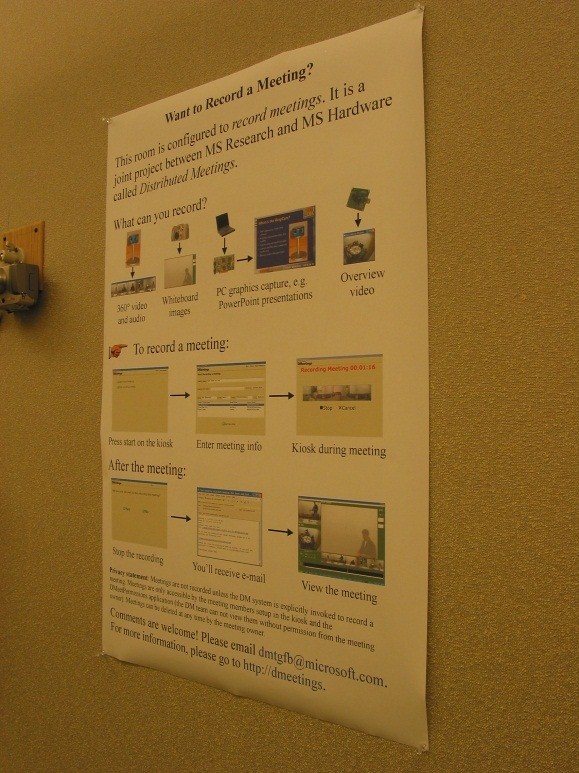
\includegraphics{images/WhiteboardIt.jpg}
			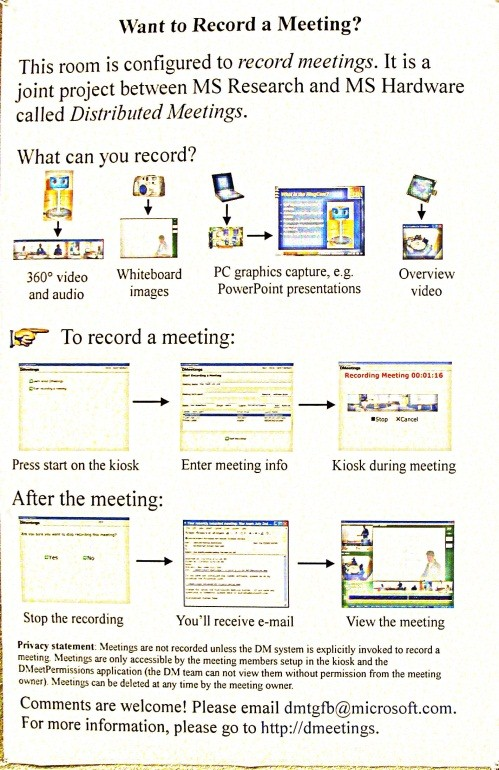
\includegraphics{images/WhiteboardIt2.jpg}\\
			
			We may wish to contact dmtgfb@microsoft.com to ask for more information on their image processing algorithms later on in the process.\\
			\\
			I’m not sure how helpful this might be, but here is a link to Ink-Enabled Apps For Tablet PC\\
			http://msdn.microsoft.com/en-us/magazine/cc967278.aspx\\
			\\
			http://www.fxpal.com/?p=reboard\\
			http://arxiv.org/abs/0911.0039\\
			The following is a paper that talk about another whiteboard captureing technology called ReBoard:\\
			http://arxiv.org/ftp/arxiv/papers/0911/0911.0039.pdf\\
			http://www.fxpal.com/publications/FXPAL-PR-10-546.pdf\\
			
		\subsection{Additional Apps:}
			\begin{itemize}
				\item Whiteboard Capture
				\item Whiteboard Share
				\item WBConference
				\item Whiteboard Snap
				\item BoardTable
			\end{itemize}

	
	% Third Entry
	\section{09/11/2012}
		I first uploaded pictures to the website for our personal biographies.
		\\
		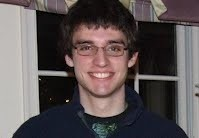
\includegraphics{images/Griffin.jpg}
		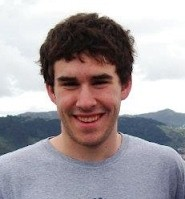
\includegraphics{images/Colin.jpg}
		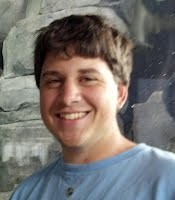
\includegraphics{images/Phil.jpg}
		\\
					After this I wrote an overview about ProPANE on our front page:\\
			Welcome to the website for the Electrical and Computer Engineering senior design project led by Griffin Dunn, Phil Stahlfeld, and Colin Madigan.
			ProPANE's goal is to design and implement a system that will automatically capture all information written on a board during class. This system will then present the saved information in a readily accessible manner so that Bucknell can both better meet the needs of students with disabilities and provide professors with a means to easily compare their notes with the actual information presented in a lecture.
			This project was motivated by Bucknell’s desire to cheaply meet the needs of their students with disabilities. Hiring professional note takers is an expensive endeavor and finding cheaper alternatives is much more desirable.
			This project involves the capture of information from a 2D surface. It will likely require image capture and image processing technology.
		\subsection{Design Constraints}
			\begin{itemize}			
				\item ProPANE must be fully autonomous. After setup the system should require little to no outside interference. The professor should be able to turn it on and leave it running during class and afterwards return to find a set of images depicting everything that was on the board during class.
				\item The information must be presented in a format that allows for easy manipulation, zooming, and editing so that students with disabilities can easily view all content that is displayed on the board.
				\item The system must be discreet. It cannot make loud noises, flashes of light, or create any other forms of distraction during class. Students must be able to concentrate on the lecture not the board capture device.
			\end{itemize}

	
	
	% Second Entry
	\section{Individual Work on Competing Technologies 09/05/2012}
		We have three technologies to compete with: 
		
		\subsection{The Phone App}
			There are several smartphone apps out there that will scan pictures of white boards and filter out the unnecessary information. These applications range from free to a couple dollars on most app stores.\\
				http://www.beetlebugsoftware.com/ is a good example. \\

				Other notable apps:
					\begin{itemize}
						\item Qipit White
						\item Genius Scan
						\item JotNot Scanner Pro
						\item Whiteboard Capture Pro
					\end{itemize}

			However, this IS an issue because it is an area that could possibly pose legal problems. If the resolution is too poor, then the system would be giving ProPANE reliant students a disadvantage. In my opinion, that would be a complete failure of the project.\\
			
		\subsection{Scanners}
			There are scanners that you can attach to an existing white board. After calibrating these scanners, they track your movements using the combination of the sanner and an electronic pen. These electronic pens have replaceable dry erase tips to draw with and replaceable batteries to keep them charged. Some of them require a projector to display background information and others do not.\\

			Examples:
				\begin{itemize}
					\item MimoCapture
					\item eBeam System 3
					\item Interlink FreeBeam
				\end{itemize}

			
		\subsubsection{Electronic Whiteboards}
			Electronic whiteboards are special boards that sense pressure and can display electronic pen interactions with a high degree of accuracy. These displays come in two standard varieties: Those that are electronic displays and those that require a projector to project both the images and any user-inputted writing. Electronic whiteboards tend to be the easiest to use, but they're not very portable because the entire board is required. The trade-off for poor portability is that they can do much more. Multiple people can interact with the board at the same time, and it can be a much more interactive experience. \\

			Examples:
			\begin{itemize}
				\item Smarttech’s SMARTboard 
				\item Panasonic’s Panaboard 
				\item Hitachi’s Starboard 
				\item The Promethean board 
			\end{itemize}

	
	%First Entry
	\section{Initial Group Meeting 08/30/2012}
			\emph{With Phil Stahlfeld and Colin Madigan}\\
			
			Began working on group tasks:
			\begin{itemize}
				\item Team Name
				\item Team Logo
				\item Document Template
				\item Design Specifications
			\end{itemize}
			
		\subsection{Team Name}
			After some discussion we decided that names such as ‘White board scanner’ and ‘board capture system’ weren’t catchy enough. We decided to create an acronym instead so to make our name catchier and thus more memorable. Colin finally came up with our final acronym: ProPANE, short for Professional Portable Automatic Note Extractor. With this agreed upon we moved on to deciding upon our team logo. \\

		\subsection{Team Logo}
			We decided that our logo had to relate to our team name, so with that in mind we searched for images related to the molecular structure of propane. Our favorite image is shown below, and has been adopted as our team logo:\\
			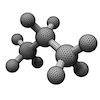
\includegraphics{images/logo.jpeg}\\

		\subsection{Document Template}
			We decided to use LaTEX as our default layout manager for all of our documents. We chose this formatter because it takes care of all the formatting and leaves us with the job of finding and preparing the information, which is the more important part of our job. 

		\subsection{Technical Specifications}
			As noted in our first deliverable, “The goal of this project is to create a system that captures all of the information written on a board during a class in a readily accessible manner. The two driving forces behind solving this problem are: autonomous collection of notes for students with disabilities and providing a means for professors to compare their notes with the actual information presented during a lecture.” \\

			We will be meeting with Robert Midkiff and Douglas Gabauer on 09/13/2013 to discuss more detailed specifications for the project.\\

		
	
	
\end{document}
